\section{Meißner-Ochsenfeld-Effekt}
Ein weiteres Phänomen der Supraleitung ist der Meißner-Ochsenfeld-Effekt. FRITZ WALTER MEIßNER und 
ROBERT OCHSENFELD entdeckten 1933, dass Magnetfelder aus dem Inneren eines Supraleiters verdrängt werden. 
Dieser Effekt tritt auf, wenn ein Supraleiter unter seine kritische Temperatur abgekühlt wird. Somit sind 
Supraleiter nicht nur ideale Leiter, sondern auch perfekte Diamagneten.
\begin{figure}[!h]
    \centering
    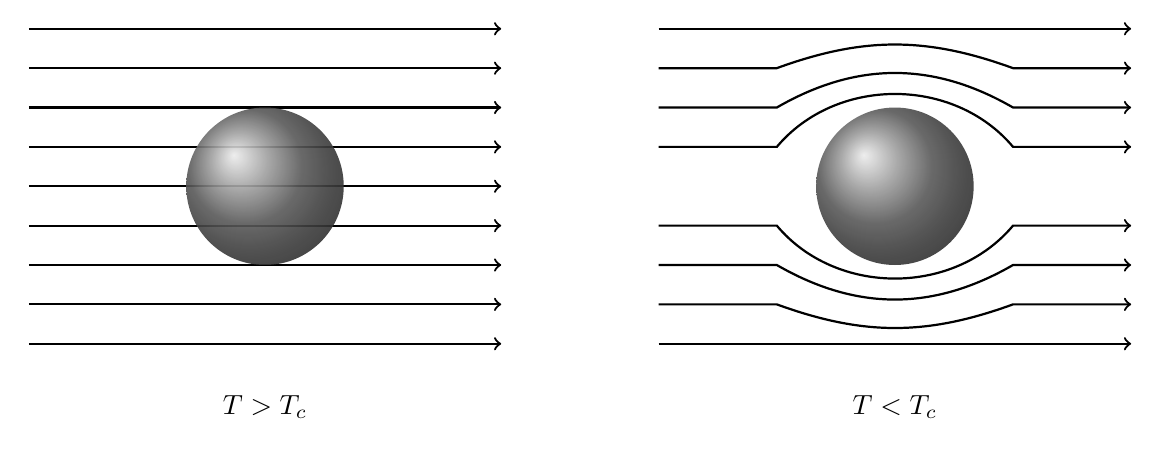
\begin{tikzpicture}
        % Left diagram: T > Tc
        \begin{scope}[xshift=-4cm]
            
            
            % Magnetic field lines (straight)
            \foreach \y in {-2, -1.5, -1, -0.5, 0, 0.5, 1, 1.5, 2} {
                \draw[thick, ->] (-3,\y) -- (3,\y);
            }
            % Ball
            \shade[ball color=gray, opacity=0.9] (0,0) circle (1);
            
            % Label
            \node at (0,-2.8) {\(T > T_c\)};
        \end{scope}
        
        % Right diagram: T < Tc
        \begin{scope}[xshift=4cm]
            % Streamlines that curve around the ball
            \draw [thick, ->] (-3, -2) -- (3,-2);
            \draw [thick, ->] (-3, -1.5) -- (-1.5,-1.5) to[out=-20, in=-160] (1.5,-1.5) -- (3,-1.5);
            \draw [thick, ->] (-3, -1) -- (-1.5,-1) to[out=-30, in=-150] (1.5,-1) -- (3,-1);
            \draw [thick, ->] (-3, -0.5) -- (-1.5,-0.5) to[out=-50, in=-130] (1.5,-0.5) -- (3,-0.5);
            %\draw [thick, ->] (-3, 0) -- (3,0);
            \draw [thick, ->] (-3, 0.5) -- (-1.5,0.5) to[out=50, in=130] (1.5,0.5) -- (3,0.5);
            \draw [thick, ->] (-3, 1) -- (-1.5,1) to[out=30, in=150] (1.5,1) -- (3,1);
            \draw [thick, ->] (-3, 1.5) -- (-1.5,1.5) to[out=20, in=160] (1.5,1.5) -- (3,1.5);
            \draw [thick, ->] (-3, 2) -- (3,2);
            
            % Ball
            \shade[ball color=gray, opacity=0.9] (0,0) circle (1);
            
            % Label
            \node at (0,-2.8) {\(T < T_c\)};
        \end{scope}
    \end{tikzpicture}
    \caption{Meißner-Ochsenfeld-Effekt}
\end{figure}

Nimmt man ein Superleitendes Material mit einer Temperatur höher als die kritische Temperatur $T_c$
und setzt es einem Magnetfeld aus, so dringt das Magnetfeld nahezu ungehindert durch das Material (wie links in Abbildung 3 zusehen ist). 
Wenn man den Supraleiter jetzt unter die kritische Temperatur abkühlt, wird das Magnetfeld aus dem Inneren des Supraleiters verdrängt (Abbildung 3 rechts).
Doch eigentlich müsste doch das Magnetfeld weiterhin ungehindert das Material durchdringen können, da der 
Widerstand gleich null ist, kann keine Spannung abfallen oder induziert werden, wodurch sich das Magnetfeld 
eigentlich nicht verändern dürfte.

Die Erklärung für dieses Phänomen ist die Londonsche Eindringtiefe. FRITZ und HANS LONDON
versuchten 1935 die charakteristischen Eigenschaften der Supraleitung durch ihre London-Gleichungen 
zu beschreiben. Daraus folgte dann das ein äußeres Magnetfeld doch in eine dünne Oberflächenschicht des Supraleiters eindringt (Eindringtiefe $\lambda_L$).

\begin{equation}
    \vec{B}(x) = \vec{B}_0 e^{-\frac{x}{\lambda_L}}
\end{equation}

Dabei ist $\vec{B}$ das Magnetfeld im Supraleiter, $\vec{B}_0$ das Magnetfeld außerhalb des Supraleiters, $d$ die Tiefe in den Supraleiter und $\lambda_L$ die Londonsche Eindringtiefe.
\\
\\
Das Magnetfeld, welches in diese dünne Schicht eindringt, führt zu einem supraleitendem Stromfluss, welcher ein
Magnetfeld erzeugt, was gerade so stark ist um das äußere Magnetfeld aufzuheben, was 
die Begründung für den Meißner-Ochsenfeld-Effekt ist. 

